\documentclass{article}

\usepackage{microtype}
\usepackage{graphicx}
\usepackage{hyperref}
\usepackage{icml2026}
\makeatletter
\renewcommand{\icmlruler}[1]{}
\makeatother
\usepackage{amsmath,amssymb}
\usepackage{booktabs}
\usepackage{array}
\usepackage{tabularx}
\usepackage{xcolor}
\usepackage{enumitem}
\usepackage{float}
\usepackage{adjustbox}
\usepackage[section]{placeins}
\usepackage{tikz}
\usetikzlibrary{arrows.meta,positioning}
\icmltitlerunning{Offline-to-Deployed Selection Transfer}

\begin{document}

\twocolumn[
  \icmltitle{Auditing Offline-to-Deployed Selection Transfer under Fixed Decision Interfaces}

  % For an anonymous ICML submission, keep the package line above as
  % \usepackage{icml2026}. To render author names in a visible draft,
  % switch it to \usepackage[preprint]{icml2026} or
  % \usepackage[accepted]{icml2026}.
  % First author requested by the user: 김금영.
  \begin{icmlauthorlist}
    \icmlauthor{Kim Geum-Young}{cbnu}
  \end{icmlauthorlist}

  \icmlaffiliation{cbnu}{School of Computer Sience, Chungbuk National University, Cheongju, Chungcheongbuk-do, South Korea}
  \icmlcorrespondingauthor{Kim Geum-Young}{anon.email@domain.com}
  \icmlkeywords{Offline decision-making, model selection, deployment-aware evaluation}

  \vskip 0.3in
]

\printAffiliationsAndNotice{}

\begin{abstract}
Offline decision-making pipelines often select models using validation scores computed on collected data, then deploy the selected model through a fixed decision interface such as threshold alerts, hysteresis rules, budgeted top-\(k\) actions, residual-warning screens, or replenishment rules. We ask a narrow evaluation question: does the offline-selected model remain the deployed-utility winner after the same interface and deployment friction are applied? We propose an offline-to-deployed selection-transfer report card that records the offline-selected model, deployed-utility winner, agreement rate, deployed-suboptimal share, paired utility shortfall, and tie diagnostics. Across the studied tasks, the offline-selected model often fails to remain the deployed-utility winner once switching or adjustment costs are applied through the fixed interface, and the mismatch recurs across seeds and interface checks. We position this report card as a pre-adaptation evaluation layer for offline decision-making pipelines: before deployment, online fine-tuning, or exploration, practitioners can audit whether the candidate selected by an offline proxy remains preferred under the fixed decision interface and friction model they intend to use.
\end{abstract}

\section{Introduction}

Offline decision-making pipelines often select a model using validation scores computed on collected data, then deploy the selected model through a fixed decision interface that maps predictions or scores into actions. Examples include triggering an alert when \(p_t > \tau\), changing state only if the score moves by at least \(\delta\), issuing the top-\(k\) alerts under a fixed budget, applying a residual-warning screen, or applying a replenishment rule. When the deployed interface includes switching or adjustment friction, the model selected by the offline score need not remain the deployed-utility winner. We do not tune the interface per model: the same specified decision interface is applied to every candidate model before deployed-utility scoring.

This paper studies offline-to-deployed selection transfer as a reporting diagnostic. By selection transfer we mean whether the model selected by an offline validation score remains the best model under deployed utility after a fixed decision interface and friction model are applied. This is not an argument that forecast-quality metrics are invalid for prediction, nor a proposal for a single deployed metric. Deployed utility depends on a specified interface, simulator, and friction model. Our claim is narrower: when offline validation is used as deployment-facing model-selection advice, the evaluation should report whether that selection transfers to deployed utility under the specified fixed interface.

In offline decision-making terms, each candidate prediction model \(f_m\), together with the fixed interface \(I_\theta\), induces a candidate decision rule \(\pi_m=I_\theta\circ f_m\). The report card is therefore a fixed-candidate selection audit: it asks whether the candidate chosen by an offline proxy score is also preferred by deployed utility under the intended interface and friction model. In many offline decision-making settings, the first deployment decision is not how to update a policy online, but which offline-trained candidate is reliable enough to deploy, evaluate, or adapt. Our report card targets this pre-adaptation selection step.

This audit is complementary to OPE, decision-focused learning, and online adaptation: those methods estimate policy value, optimize downstream objectives, or adapt policies online, whereas our report card checks whether a fixed offline-selected candidate remains preferred under the intended interface and friction model.

\begin{figure*}[t]
\centering
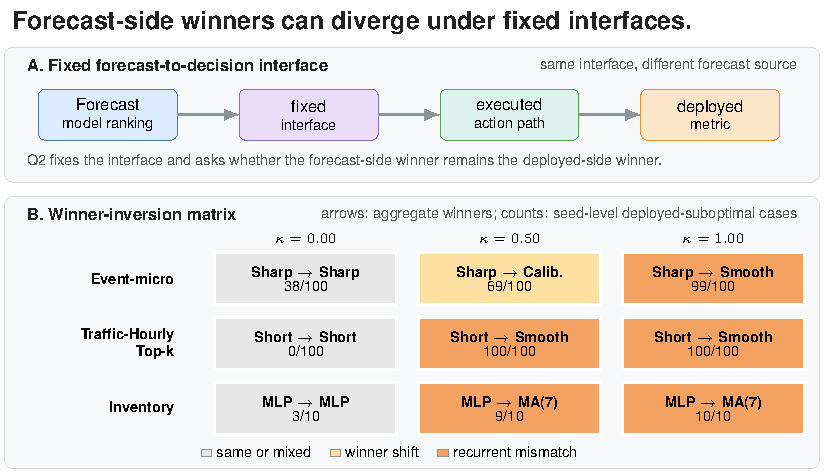
\includegraphics[width=0.98\textwidth]{assets/figures/fig1_fixed_interface_inversion.pdf}
\caption{Offline-selected candidates can lose after fixed-interface deployment. (A) The audit ranks candidate models offline, applies the same fixed interface, and scores deployed utility under friction. (B) Arrows show offline-selected candidate \(\rightarrow\) deployed-utility winner; counts show deployed-suboptimal units. Gray cells are zero-friction references, not friction-causal evidence.}
\label{fig:fixed-interface-inversion}
\end{figure*}

This paper makes three focused contributions.
\begin{itemize}[leftmargin=*,noitemsep,topsep=2pt]
\item Selection-transfer diagnostic. We formulate offline-to-deployed selection-transfer robustness: whether the model selected by an offline validation score remains the best model under deployed utility after a fixed decision interface and friction model are applied.
\item Report-card artifact. We provide a lightweight report card recording offline-selected models, deployed-utility winners, agreement rates, deployed-suboptimal shares, paired utility shortfalls, and tie/uncertainty diagnostics.
\item Empirical audit. Across prediction-to-decision tasks, we find recurrent selection failures in the tested higher-friction settings, while retaining zero-friction anchors, failed-gate variants, and tie audits to bound the interpretation.
\end{itemize}

\paragraph{Setup.}
For each candidate model \(m \in \mathcal{M}\), an offline validation score \(S_{\mathrm{off}}(m)\) selects \(m_{\mathrm{off}}=\arg\min_m S_{\mathrm{off}}(m)\). We use the loss convention for \(S_{\mathrm{off}}\), with lower values better. A fixed decision interface \(I_\theta\) maps model outputs to actions, \(a^m_{1:T}=I_\theta(\hat y^m_{1:T})\), and the same specified interface is applied to every candidate model. We evaluate deployed utility \(U_\kappa(m;I_\theta)\) under friction \(\kappa\), with larger values better. The deployed-utility winner is \(m_{\mathrm{dep}}=\arg\max_m U_\kappa(m;I_\theta)\). Selection transfer is preserved when \(m_{\mathrm{off}}=m_{\mathrm{dep}}\); otherwise the offline-selected model incurs deployed shortfall \(\Delta_\kappa=U_\kappa(m_{\mathrm{dep}};I_\theta)-U_\kappa(m_{\mathrm{off}};I_\theta)\). All deployed outcomes are reported as utilities or utility shortfalls, so larger \(U_\kappa\) is better and \(\Delta_\kappa>0\) means the offline-selected model is deployed-suboptimal. Near-ties are handled by the pre-specified tie-breaking rule and by the \(\epsilon\)-tie audit reported in the appendix. Throughout the paper, ``offline-selected model'' denotes the candidate chosen by the offline validation score; ``deployed-utility winner'' denotes the candidate with the highest utility after the same fixed interface and friction model are applied.

Q2 is the paper's main model-selection question: with the interface fixed, does the offline-selected model remain the deployed-utility winner? Q1 is used only as a mechanism check: when the proposed action path is held fixed, frictional execution can change realized utility. We report Q1 only to explain why Q2 failures can arise.

\section{Results}

\subsection{Selection transfer under fixed decision interfaces}

This subsection answers Q2: with the decision interface fixed, does the offline-selected model remain the deployed-utility winner? Table~\ref{tab:deployed-selection-report-card} reports the resulting selection-transfer report card. Event-micro and Traffic-Hourly carry the main fixed-interface selection-transfer claim; EPA and inventory are bounded support.

\begin{table*}[t]
\caption{Offline-to-deployed selection-transfer report card. Each row fixes a task, decision interface, and friction level. Transfer is the fraction of evaluation units where the offline-selected model also maximizes deployed utility; Subopt. counts the complementary deployed-suboptimal units. Shortfall is the paired deployed-utility gap to the deployed-utility winner in task-specific units, so values should be compared within, not across, task families.}
\label{tab:deployed-selection-report-card}
\centering
\scriptsize
\setlength{\tabcolsep}{2.5pt}
\begin{tabular*}{\textwidth}{@{\extracolsep{\fill}}llcllccccl@{}}
\toprule
Task & Fixed interface & $\kappa$ & Offline-selected & Deployed winner & Transfer & Subopt. & Shortfall & 95\% CI & Evidence role \\
\midrule
Synthetic & zero-friction anchor & 0.00 & Naive last & Naive last & 1.00 & 0/20 & 0.000 & [0.000, 0.000] & sanity \\
Event warning & threshold $\tau{=}0.55$ & 0.50 & Reactive sharp & Calibrated & 0.31 & 69/100 & 0.011 & [0.009, 0.014] & main Q2 \\
Event warning & threshold $\tau{=}0.55$ & 1.00 & Reactive sharp & Smoother & 0.01 & 99/100 & 0.057 & [0.052, 0.063] & main Q2 \\
Budgeted traffic alert & budget $k{=}249$ & 0.50 & Reactive short & Smoother & 0.00 & 100/100 & 7.02 & [6.76, 7.28] & supporting Q2 \\
Budgeted traffic alert & budget $k{=}249$ & 1.00 & Reactive short & Smoother & 0.00 & 100/100 & 24.65 & [24.23, 25.08] & supporting Q2 \\
PM2.5 warning & residual warning & 1.00 & Reactive lag-1 & Long smoother & 0.00 & 720/825 & 17.94 & [16.56, 19.34] & residual support \\
Inventory replenishment & replenishment & 1.00 & Small MLP & MA(7) & 0.01 & 99/100 & 1.03 & [0.95, 1.11] & operational support \\
\bottomrule
\end{tabular*}
\end{table*}

\paragraph{Why offline ordering need not be preserved.} Offline validation scores evaluate their specified validation objective, not the composed object obtained after model outputs are mapped to actions and executed through a frictional interface. If a candidate model's offline validation advantage is smaller than the extra friction-induced loss created by its implied action path, the deployed ordering can reverse even under a fixed interface.

Event-micro is the primary evidence because it isolates the selection-transfer question under a simple threshold interface and includes three robustness checks: an alternate threshold, log-loss reranking, and a hysteresis interface. In the report card, the offline-selected model remains Reactive sharp, but the deployed-utility winner changes to Calibrated baseline at friction 0.50 and Lagged smoother at friction 1.00. The deployed-utility consequence is recurrent: the offline-selected model is deployed-suboptimal in 69/100 and 99/100 seeds at these two friction levels. The result is not confined to the canonical threshold or Brier ranking: at frictions 0.50/1.00, deployed-suboptimality remains 77/100 and 98/100 under an alternate threshold, 74/100 and 99/100 under log-loss reranking, and 55/100 and 82/100 under a hysteresis interface, where the direction is preserved with smaller magnitude.

Traffic-Hourly Top-\(k\) is a prediction-to-decision task: forecasts are ranked by an offline validation score, but the fixed interface deploys only the top-\(k\) actions under a budget. The Traffic-Hourly pattern is not isolated to the canonical budget: appendix heatmaps show the same zero-friction alignment and positive-friction mismatch across \(k \in \{125,249,500,750\}\) and across canonical, earlier, and later temporal splits. In the selected Top-\(k\) setting ($k=249$), Reactive short is both the offline-selected model and the deployed-utility winner at zero friction, with exact transfer $1.0$. Once switching costs are introduced, however, the offline-selected model remains Reactive short while the deployed-utility winner shifts to Lagged smoother, and deployed-suboptimality reaches $100/100$ seeds at both friction $0.5$ and friction $1.0$.

EPA PM2.5 adds a broader residual-warning audit row without changing the evidence hierarchy. In expanded EPA AQS PM2.5 residual warning, Reactive lag-1 remains the offline-selected model, while Long smoother becomes the deployed-utility winner at \(\kappa=1.00\). We treat its units as report-card evaluation cells rather than independent iid samples. We interpret the EPA row as a broader residual-warning audit rather than independent population-level evidence; it shows that the report-card failure mode is not unique to the Event or Traffic constructions. The appendix reports the full residual-candidate audit, including appendix-only residual-audit support and failed-gate context.

An \(\epsilon\)-tie audit gives the same qualitative reading for the main prediction-to-decision rows: Traffic-Hourly Top-\(k\) and Event-micro at \(\kappa \in \{0.50,1.00\}\), and expanded EPA at \(\kappa=1.00\), remain deployed-suboptimal under relative tie thresholds up to \(\epsilon_{\mathrm{rel}}=0.005\); inventory remains corroborative and lower-margin secondary checks are reported only in the appendix.

Intervals are descriptive summaries for report-card cells, not hypothesis tests for a broader population-level claim. Appendix \(\epsilon\)-tie and mixed/failed-gate variants help guard against reading the main table as selected successes only.

Inventory is retained as operational corroboration: it shows that the same audit format applies to a replenishment interface, but it is not used as primary evidence for the offline decision-making claim. At friction 0.50 and 1.00, the offline-selected Small MLP is deployed-suboptimal in 74/100 and 99/100 seeds, respectively, under the fixed replenishment interface; the report card includes only the high-friction inventory row to keep this role bounded.

\paragraph{Q1 mechanism support.} Q1 is not the main empirical claim. It is a mechanism check using synthetic and inventory fixed-action replay: when the proposed action path is held fixed, frictional execution can separate proposed and realized actions and change realized utility. The fixed-interface Q2 rows in Table~\ref{tab:deployed-selection-report-card} provide the paper's actual selection-transfer evidence.

\paragraph{Appendix robustness.} Appendix checks are organized to answer whether the main rows are isolated successes: Event robustness varies threshold, scoring rule, and interface; Traffic robustness varies \(k\) and deployment window; mixed/failed-gate and tie-sensitivity rows are retained to show where the audit does not support a paper-facing claim. Appendix~\ref{app:reselection-diagnostic} adds a replay-based deployed-feedback diagnostic: in Traffic Top-\(k\), small calibration segments substantially reduce the observed misselection under fixed-interface replay on held-out outcomes; we keep this outside the main claim because it is not an online learning algorithm. Stronger-pool and residual-audit checks remain appendix-only, while time-of-day, relative-rank, inventory, and load-following variants are compressed as secondary context.

\section{Discussion, Related Work, and Limitations}

\paragraph{Offline policy evaluation and offline-to-deployment selection.} Policy comparison and OPE study how candidate policies can be compared before costly deployment. OPE asks whether policy value can be estimated from logged data under assumptions about coverage, propensities, or learned models. Offline-to-online adaptation asks how to update or explore after deployment begins. Our report card targets the preceding selection step: the candidate set and deployment interface are fixed, and the diagnostic asks whether the offline proxy used for candidate selection agrees with deployed utility under a specified replay/evaluation environment.

\paragraph{Decision-focused learning and predict-then-optimize.} Decision-focused learning and predict-then-optimize change the training or optimization objective to improve downstream decisions \cite{raeth2025,donti2017task,elmachtoub2021spo,mandi2024decisionfocused}. Our candidates are already trained; the contribution is a reporting layer that detects when the offline-selected candidate would be deployment-suboptimal under the intended interface.

\paragraph{Prediction benchmarks and decision-facing selection.} Forecasting benchmarks and evaluation frameworks now span live AI forecasting, broad time-series archives, foundation-model evaluations, text-conditioned forecasting, and standardized TSFM evaluation pipelines \cite{forecastbench,prophetarena,gifteval,godahewa2021monash,das2024timesfm,williams2025contextkey,tsfmbench2025,tempusbench2026,timerecipe2025}. These works compare forecasting capability, datasets, model families, or evaluation pipelines, and proper scoring rules remain the right object when the target is predictive quality \cite{gneiting2007,murphy1993}. Our question is complementary: when a prediction benchmark is interpreted as deployment-facing model-selection advice under a fixed decision interface, should it also report whether offline validation selection transfers to deployed utility?

\paragraph{Benchmark uncertainty and report-card intervals.} Our uncertainty reporting follows the spirit of benchmark-variance and leaderboard-interpretation work \cite{bouthillier2021variance,longjohn2025aggregate,fevbench2025,brigato2025nochampions}, but reports selection transfer and deployed shortfalls rather than aggregate predictive leaderboard uncertainty. Deployment frictions such as switching costs, adjustment costs, and operational churn can change which model is preferable after actions are executed; the report card makes this effect visible at the model-selection level.

\paragraph{Discussion and limitations.} Our claim is evaluative and deliberately narrow. We do not claim that forecasting metrics are invalid for prediction, and we do not seek a single reporting rule for all applications. We use low, moderate, and high only as shorthand for the lower, middle, and upper parts of each domain's tested friction grid; these labels are not intended as a universal calibration across domains. Event-micro and Traffic-Hourly provide the core fixed-interface selection-transfer evidence, the EPA residual-warning audit adds one additional report-card row, and inventory provides operational corroboration. These settings are intended as a focused audit of offline-to-deployed selection transfer, not as a comprehensive offline decision-making benchmark suite. Inventory and load-following variants are retained only as compressed secondary context; the strongest main-text evidence comes from the moderate-to-high friction settings studied here. The contribution is a fixed-interface selection-audit protocol: a lightweight pre-adaptation layer for checking whether the offline-selected candidate remains preferred before policy learning, OPE-based deployment decisions, online adaptation, or application-specific utility redesign. It is a narrow reporting recommendation: when offline validation is interpreted as model-selection advice for a fixed deployment interface, it should also report whether offline selection transfers to deployed utility. Under this interpretation, inventory and load-following remain corroborative or secondary context rather than standalone statistical evidence for a broader population-level claim.

\begingroup
\small
\setlength{\emergencystretch}{2em}
\begin{thebibliography}{99}
\bibitem[Karger et~al.(2025)Karger, Bastani, Yueh-Han, Jacobs, Halawi, Zhang, and Tetlock]{forecastbench}
E. Karger, H. Bastani, C. Yueh-Han, Z. Jacobs, D. Halawi, F. Zhang, and P. E. Tetlock.
\newblock ForecastBench: A Dynamic Benchmark of AI Forecasting Capabilities.
\newblock In \emph{ICLR}, 2025. arXiv:2409.19839.

\bibitem[Yang et~al.(2025)Yang, Mahns, Li, Gu, Wu, and Xu]{prophetarena}
Q. Yang, S. Mahns, S. Li, A. Gu, J. Wu, and H. Xu.
\newblock LLM-as-a-Prophet: Understanding Predictive Intelligence with Prophet Arena.
\newblock arXiv:2510.17638, 2025.

\bibitem[Aksu et~al.(2024)Aksu, Woo, Liu, Liu, Liu, Savarese, Xiong, and Sahoo]{gifteval}
T. Aksu, G. Woo, J. Liu, X. Liu, C. Liu, S. Savarese, C. Xiong, and D. Sahoo.
\newblock GIFT-Eval: A Benchmark for General Time Series Forecasting Model Evaluation.
\newblock NeurIPS Workshop on Time Series in the Age of Large Models, 2024. Extended version: arXiv:2410.10393.

\bibitem[Godahewa et~al.(2021)Godahewa, Bergmeir, Webb, Hyndman, and Montero-Manso]{godahewa2021monash}
R. Godahewa, C. Bergmeir, G. I. Webb, R. J. Hyndman, and P. Montero-Manso.
\newblock Monash Time Series Forecasting Archive.
\newblock In \emph{NeurIPS Datasets and Benchmarks}, 2021. arXiv:2105.06643.

\bibitem[Das et~al.(2024)Das, Kong, Sen, and Zhou]{das2024timesfm}
A. Das, W. Kong, R. Sen, and Y. Zhou.
\newblock A decoder-only foundation model for time-series forecasting.
\newblock In \emph{ICML}, 2024. OpenReview: jn2iTJas6h; arXiv:2310.10688.

\bibitem[Williams et~al.(2025)Williams, Ashok, Marcotte, Zantedeschi, Subramanian, Riachi, Requeima, Lacoste, Rish, Chapados, and Drouin]{williams2025contextkey}
A. R. Williams, A. Ashok, E. Marcotte, V. Zantedeschi, J. Subramanian, R. Riachi, J. Requeima, A. Lacoste, I. Rish, N. Chapados, and A. Drouin.
\newblock Context is Key: A Benchmark for Forecasting with Essential Textual Information.
\newblock In \emph{ICML}, PMLR 267, pages 66887--66944, 2025.

\bibitem[Li et~al.(2025)Li, Qiu, Chen, Wang, Cheng, Shu, Hu, Guo, Zhou, Jensen, and Yang]{tsfmbench2025}
Z. Li, X. Qiu, P. Chen, Y. Wang, H. Cheng, Y. Shu, J. Hu, C. Guo, A. Zhou, C. S. Jensen, and B. Yang.
\newblock TSFM-Bench: A Comprehensive and Unified Benchmark of Foundation Models for Time Series Forecasting.
\newblock arXiv:2410.11802, 2025.

\bibitem[Goktas et~al.(2026)Goktas, Riano-Briceno, Abdullah, Nair, Shen, de Lucio, Magnusson, Mashrur, Abdulla, Sen, Thippireddy, Schwartz, and Greenwald]{tempusbench2026}
D. Goktas, G. Riano-Briceno, A. Abdullah, A. Nair, C. Shen, B. de Lucio, A. Magnusson, F. Mashrur, A. Abdulla, S. Sen, M. Thippireddy, G. Schwartz, and A. Greenwald.
\newblock TempusBench: An Evaluation Framework for Time-Series Forecasting.
\newblock arXiv:2604.11529, 2026.

\bibitem[Zhao et~al.(2025)Zhao, Ni, Xu, Liu, Jin, and Prakash]{timerecipe2025}
Z. Zhao, J. Ni, S. Xu, H. Liu, W. Jin, and B. A. Prakash.
\newblock TimeRecipe: A Time-Series Forecasting Recipe via Benchmarking Module Level Effectiveness.
\newblock arXiv:2506.06482, 2025.

\bibitem[Bouthillier et~al.(2021)Bouthillier, Delaunay, Bronzi, Trofimov, Nichyporuk, Szeto, Sepah, Raff, Madan, Voleti, Kahou, Michalski, Arbel, Pal, Varoquaux, and Vincent]{bouthillier2021variance}
X. Bouthillier, P. Delaunay, M. Bronzi, A. Trofimov, B. Nichyporuk, J. Szeto, N. Sepah, E. Raff, K. Madan, V. Voleti, S. E. Kahou, V. Michalski, T. Arbel, C. Pal, G. Varoquaux, and P. Vincent.
\newblock Accounting for Variance in Machine Learning Benchmarks.
\newblock In \emph{MLSys}, 2021. arXiv:2103.03098.

\bibitem[Longjohn et~al.(2025)Longjohn, Gopalan, and Casleton]{longjohn2025aggregate}
R. Longjohn, G. Gopalan, and E. Casleton.
\newblock Statistical Uncertainty Quantification for Aggregate Performance Metrics in Machine Learning Benchmarks.
\newblock arXiv:2501.04234, 2025.

\bibitem[Shchur et~al.(2025)Shchur, Ansari, Turkmen, Stella, Erickson, Guerron, Bohlke-Schneider, and Wang]{fevbench2025}
O. Shchur, A. F. Ansari, C. Turkmen, L. Stella, N. Erickson, P. Guerron, M. Bohlke-Schneider, and Y. Wang.
\newblock fev-bench: A Realistic Benchmark for Time Series Forecasting.
\newblock arXiv:2509.26468, 2025.

\bibitem[Brigato et~al.(2026)Brigato, Morand, Strommen, Panagiotou, Schmidt, and Mougiakakou]{brigato2025nochampions}
L. Brigato, R. Morand, K. J. Strommen, M. Panagiotou, M. Schmidt, and S. Mougiakakou.
\newblock There are no Champions in Supervised Long-Term Time Series Forecasting.
\newblock \emph{Transactions on Machine Learning Research}, 2026. arXiv:2502.14045.

\bibitem[Gneiting and Raftery(2007)]{gneiting2007}
T. Gneiting and A. E. Raftery.
\newblock Strictly Proper Scoring Rules, Prediction, and Estimation.
\newblock \emph{Journal of the American Statistical Association}, 102(477):359--378, 2007.

\bibitem[Murphy(1993)]{murphy1993}
A. H. Murphy.
\newblock What Is a Good Forecast? An Essay on the Nature of Goodness in Weather Forecasting.
\newblock \emph{Weather and Forecasting}, 8(2):281--293, 1993.

\bibitem[Raeth and Ludwig(2025)]{raeth2025}
K. Raeth and N. Ludwig.
\newblock Evaluating Weather Forecasts from a Decision Maker's Perspective.
\newblock arXiv:2512.14779, 2025.

\bibitem[Donti et~al.(2017)Donti, Amos, and Kolter]{donti2017task}
P. L. Donti, B. Amos, and J. Zico Kolter.
\newblock Task-based End-to-end Model Learning in Stochastic Optimization.
\newblock In \emph{NeurIPS}, 2017. arXiv:1703.04529.

\bibitem[Elmachtoub and Grigas(2022)]{elmachtoub2021spo}
A. N. Elmachtoub and P. Grigas.
\newblock Smart ``Predict, then Optimize''.
\newblock \emph{Management Science}, 68(1):9--26, 2022.

\bibitem[Mandi et~al.(2024)Mandi, Kotary, Berden, Mulamba, Bucarey, Guns, and Fioretto]{mandi2024decisionfocused}
J. Mandi, J. Kotary, S. Berden, M. Mulamba, V. Bucarey, T. Guns, and F. Fioretto.
\newblock Decision-Focused Learning: Foundations, State of the Art, Benchmark and Future Opportunities.
\newblock \emph{Journal of Artificial Intelligence Research}, 81:1623--1701, 2024. doi:10.1613/jair.1.15320.
\end{thebibliography}
\endgroup

\clearpage
\appendix
\onecolumn

\setcounter{figure}{0}
\setcounter{table}{0}
\renewcommand{\thefigure}{A\arabic{figure}}
\renewcommand{\thetable}{A\arabic{table}}
\renewcommand{\theHfigure}{A\arabic{figure}}
\renewcommand{\theHtable}{A\arabic{table}}

\captionsetup{font=footnotesize}
\setlength{\floatsep}{6pt plus 2pt minus 2pt}
\setlength{\textfloatsep}{7pt plus 2pt minus 2pt}
\setlength{\intextsep}{7pt plus 2pt minus 2pt}
\setlength{\abovecaptionskip}{3pt}
\setlength{\belowcaptionskip}{0pt}

\providecommand{\appfigwidth}{0.92\linewidth}
\providecommand{\appwidefigwidth}{0.98\linewidth}
\providecommand{\appwidetablewidth}{0.92\linewidth}
\providecommand{\appmidtablewidth}{0.80\linewidth}
\providecommand{\appnarrowtablewidth}{0.79\linewidth}
\providecommand{\appcontexttablewidth}{\appmidtablewidth}
\providecommand{\apptablesize}{\small}
\providecommand{\apptighttablesize}{\footnotesize}

\setlength{\tabcolsep}{3.6pt}
\renewcommand{\arraystretch}{1.00}

\begin{center}
\fbox{
\begin{minipage}{0.93\linewidth}
\noindent\textbf{Minimum reporting standard for offline-to-deployed selection transfer.}\par
\smallskip
\noindent For each task family, the report-card artifact records:
\begin{enumerate}[leftmargin=*,label=\arabic*.,align=left,widest=11,itemsep=2pt,topsep=3pt,parsep=0pt]
\item task definition, seed count, and evaluation split;
\item offline validation score and tie-breaking rule;
\item fixed decision interface and interface parameters;
\item friction grid, including a zero-friction anchor and its status when applicable;
\item candidate model families and representative selection rule;
\item split/seed manifest;
\item offline-selected model and deployed-utility winner for each domain $\times$ interface $\times$ friction cell;
\item agreement rate and deployed-suboptimal share/count of the offline-selected model;
\item mean and median paired deployed-utility shortfalls with uncertainty intervals;
\item uncertainty and $\epsilon$-tie audit;
\item mixed or failed-gate variants, when applicable.
\end{enumerate}
\end{minipage}
}
\end{center}

\begin{table}[!htbp]
\centering
\begin{minipage}{\appnarrowtablewidth}
\centering
\scriptsize
\setlength{\tabcolsep}{3pt}
\renewcommand{\arraystretch}{0.95}
\begin{tabular}{p{0.23\linewidth}p{0.22\linewidth}p{0.22\linewidth}p{0.23\linewidth}}
\toprule
Concern & Appendix evidence & Concern & Appendix evidence \\
\midrule
threshold sensitivity & Event alternate \(\tau\) & top-\(k\) sensitivity & Traffic \(k\)-grid heatmap \\
offline metric sensitivity & Event log-loss reranking & temporal robustness & Traffic canonical/earlier/later splits \\
interface sensitivity & Event hysteresis & cherry-picking concern & Mixed/failed-gate variants \\
near-tie concern & \(\epsilon\)-tie audit & residual-warning generality & EPA/Capital/Wikimedia plus failed NYC/M5 \\
\bottomrule
\end{tabular}
\caption{Review-facing robustness map. Each row links a common interpretation concern to the appendix diagnostic that bounds it.}
\label{tab:review_facing_robustness_map}
\end{minipage}
\end{table}

Some generated appendix tables use legacy column labels for the offline-selected model and deployed-utility winner; the surrounding captions define their paper-facing meaning.

\paragraph{Audit-status labels.}
Audit-status labels are descriptive shorthands rather than hypothesis-test outcomes.
A row is marked \emph{Pass} when the intended zero-friction or reference-alignment check is satisfied, positive-friction deployed-suboptimality is recurrent, paired deployed-utility shortfalls are positive with descriptive uncertainty intervals, and the result is not removed by the \(\epsilon\)-tie audit when applicable.
\emph{Boundary} denotes directionally consistent but lower-margin, transition-region, partially recurrent, or partially tie-sensitive behavior.
\emph{Fail} denotes failed zero-friction alignment, lack of recurrence, or behavior dominated by objective mismatch rather than friction-induced selection-transfer failure.
For diagnostic-specific tables, such as replay-based deployed-feedback reselection and \(\epsilon\)-tie sensitivity, status labels are local to the diagnostic and are defined by the corresponding caption.

\paragraph{Mixed and failed-gate variants.}
We retain mixed and failed-gate variants as audit evidence rather than promoting them into the main report card. This reduces the risk that the report card is read as a collection of selected successes: variants that fail the zero-friction alignment check, remain lower-margin under tie diagnostics, or show only partial recurrence are kept as appendix context or excluded from main-text claims.

\begin{table}[!htbp]
\centering
\begin{minipage}{\appnarrowtablewidth}
\centering
\scriptsize
\setlength{\tabcolsep}{3pt}
\renewcommand{\arraystretch}{0.98}
\begin{tabular}{p{0.25\linewidth}p{0.20\linewidth}p{0.32\linewidth}p{0.15\linewidth}}
\toprule
Variant & Audit status & Interpretation & Placement \\
\midrule
Traffic daytime $\kappa=0.5$ & Boundary & Lower-margin, directionally consistent & Appendix only \\
Inventory zero/low friction & Mixed & Not a main zero-friction anchor & Appendix only \\
Expanded inventory & Mixed & Fairness context only & Appendix only \\
Load-alert screening & Boundary/Fail & Daily peak-hour Boundary; residual/four-week Fail & Screening artifacts \\
Residual-candidate audit & Mixed & Expanded EPA/Capital/Wikimedia pass; NYC/M5 fail zero-friction alignment & Appendix~\ref{app:residual-audit} \\
\bottomrule
\end{tabular}
\caption{Mixed, boundary, and failed-gate variants retained as audit context. These variants are not promoted into the main report card because they either fail the clean zero-friction alignment check, show lower-margin or tie-sensitive behavior, or provide only partial recurrence.}
\label{tab:mixed_failed_gate_variants}
\end{minipage}
\end{table}

These variants are useful because they separate friction-induced selection-transfer failure from other sources of mismatch, such as objective mismatch, weak margins, or insufficient seed support. We therefore use them to bound the interpretation rather than to strengthen the main claim.

\section{Event-Warning Decision Task Robustness}
\label{app:event-micro}

Because event-micro provides the paper's main prediction-to-decision selection-transfer evidence, this appendix records the first domain-specific robustness package for that benchmark. We construct a minimal binary-event setting evaluated over 100 seeds, in which each candidate prediction model emits event probabilities, a fixed thresholding rule maps probabilities to actions, and switching friction penalizes action changes. The main text uses Brier as the canonical offline validation score. This appendix records the canonical six-row Brier summary plus an alternate-threshold check, a log-loss reranking check, and a second-interface hysteresis check.

\begin{figure}[!htbp]
\centering
\begin{minipage}[c]{0.46\linewidth}
\centering
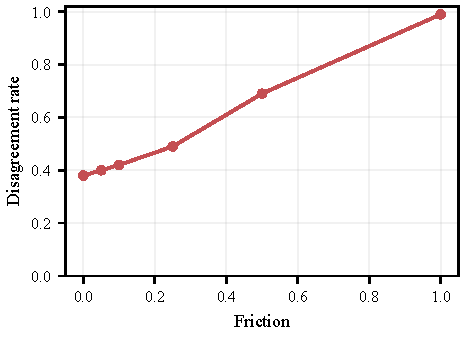
\includegraphics[width=\linewidth]{assets/figures/fig_q2_event_micro_support_compact.pdf}
\end{minipage}
\hspace{0.035\linewidth}
\begin{minipage}[c]{0.41\linewidth}
\centering
\footnotesize
\setlength{\tabcolsep}{3pt}
\begin{tabular}{ccccc}
\toprule
\(\kappa\) & \shortstack{Offline-\\selected} & \shortstack{Deployed\\winner} & Transfer & Shortfall \\
\midrule
0.00 & Sharp & Sharp & 0.62 & 0.003 \\
0.05 & Sharp & Sharp & 0.60 & 0.002 \\
0.10 & Sharp & Sharp & 0.58 & 0.002 \\
0.25 & Sharp & Calibrated & 0.51 & 0.003 \\
0.50 & Sharp & Calibrated & 0.31 & 0.011 \\
1.00 & Sharp & Smoother & 0.01 & 0.057 \\
\bottomrule
\end{tabular}
\end{minipage}
\caption{Event-micro canonical summary. Left: disagreement between offline and deployed-utility model selection increases with friction. Right: canonical fixed-threshold selection summary; shortfall is the mean paired deployed-utility shortfall of the offline-selected model.}
\label{fig:event-micro-canonical-summary}
\end{figure}

\begin{table}[!htbp]
\centering
\scriptsize
\setlength{\tabcolsep}{2.5pt}
\begin{adjustbox}{width=\appwidetablewidth}
\input{results/table_q2_selection_drift_event_micro_threshold_robustness.tex}
\end{adjustbox}
\caption{Alternate-threshold robustness for the event-micro benchmark. The same qualitative selection-transfer mismatch and recurrent deployed-suboptimality pattern persists when the fixed threshold is changed from $\tau = 0.55$ to $\tau = 0.50$.}
\label{tab:event-micro-threshold-robustness}
\end{table}

\begin{table}[!htbp]
\centering
\scriptsize
\setlength{\tabcolsep}{2.5pt}
\begin{adjustbox}{width=\appwidetablewidth}
\begin{tabular}{lllllll}
\toprule
Friction & Forecast-side winner & Deployed winner & Agreement rate & Mean deployed gap & Median deployed gap & Deployed-suboptimal seeds / total \\
\midrule
0.00 & Reactive sharp & Reactive sharp & 0.62 & 0.002 & 0.000 & 38/100 \\
0.50 & Reactive sharp & Calibrated baseline & 0.26 & 0.013 & 0.010 & 74/100 \\
1.00 & Reactive sharp & Lagged smoother & 0.01 & 0.060 & 0.057 & 99/100 \\
\bottomrule
\end{tabular}

\end{adjustbox}
\caption{Log-loss robustness for the event-micro benchmark at the canonical threshold. The same qualitative selection-transfer mismatch and recurrent deployed-suboptimality pattern persists when offline validation ranking is recomputed with log loss instead of Brier.}
\label{tab:event-micro-logloss-robustness}
\end{table}

\begin{table}[!htbp]
\centering
\scriptsize
\setlength{\tabcolsep}{2.5pt}
\begin{adjustbox}{width=\appwidetablewidth}
\begin{tabular}{llllllll}
\toprule
Interface & Friction & Forecast-side winner & Deployed winner & Agreement rate & Mean deployed gap & Median deployed gap & Deployed-suboptimal seeds / total \\
\midrule
Hysteresis threshold & 0.00 & Reactive sharp & Reactive sharp & 0.55 & 0.003 & 0.000 & 45/100 \\
Hysteresis threshold & 0.50 & Reactive sharp & Calibrated baseline & 0.45 & 0.005 & 0.001 & 55/100 \\
Hysteresis threshold & 1.00 & Reactive sharp & Lagged smoother & 0.18 & 0.022 & 0.020 & 82/100 \\
\bottomrule
\end{tabular}

\end{adjustbox}
\caption{Second-interface robustness for the event-micro benchmark. Under a fixed hysteresis-threshold interface with $\delta = 0.05$, the same qualitative selection-transfer mismatch and deployed-suboptimality pattern remains visible, though the magnitudes are smaller than under the canonical fixed threshold.}
\label{tab:event-micro-hysteresis-robustness}
\end{table}

Across this appendix robustness package, the same qualitative selection-transfer mismatch and recurrent deployed-suboptimality pattern persists in a minimal prediction-to-decision event-micro benchmark evaluated over 100 seeds.

\subsection{Interface-Aware Event-Micro Stats Addendum}
\label{app:event-micro-interface-stats}

This addendum records interface-specific recurrence and gap summaries for the hysteresis-threshold check without changing the main cross-domain recurrence package.

\begin{table}[!htbp]
\centering
\begin{minipage}{\appmidtablewidth}
\centering
\scriptsize
\setlength{\tabcolsep}{2.5pt}
\begin{adjustbox}{width=\linewidth}
\begin{tabular}{lllllll}
\toprule
Interface & $\kappa$ & Seeds & Agree. & Subopt. share/count & Subopt. 95\% CI & CI type \\
\midrule
Fixed threshold & 0.50 & 100 & 0.31 & 0.69 (69/100) & [0.594, 0.772] & Wilson \\
Fixed threshold & 1.00 & 100 & 0.01 & 0.99 (99/100) & [0.946, 0.998] & Wilson \\
Hysteresis threshold & 0.50 & 100 & 0.45 & 0.55 (55/100) & [0.452, 0.644] & Wilson \\
Hysteresis threshold & 1.00 & 100 & 0.18 & 0.82 (82/100) & [0.733, 0.883] & Wilson \\
\bottomrule
\end{tabular}

\end{adjustbox}
\caption{Interface-aware recurrence and share uncertainty for event-micro deployed-suboptimality. The canonical fixed threshold shows stronger recurrence, while hysteresis preserves the same direction with smaller magnitudes.}
\label{tab:event-micro-interface-recurrence-tests}
\end{minipage}
\end{table}

The aggregate recurrence table reports the seed-level pattern directly, replacing the dense seed-strip visualization.

\begin{table}[!htbp]
\centering
\scriptsize
\setlength{\tabcolsep}{2.5pt}
\begin{adjustbox}{width=\appwidetablewidth}
\begin{tabular}{llllll}
\toprule
Interface & Friction & Mean deployed gap & Mean gap 95\% bootstrap CI & Median deployed gap & Median gap 95\% bootstrap CI \\
\midrule
Fixed threshold & 0.50 & 0.011 & [0.009, 0.014] & 0.008 & [0.004, 0.011] \\
Fixed threshold & 1.00 & 0.057 & [0.052, 0.063] & 0.053 & [0.048, 0.059] \\
Hysteresis threshold & 0.50 & 0.005 & [0.004, 0.006] & 0.001 & [0.000, 0.003] \\
Hysteresis threshold & 1.00 & 0.022 & [0.019, 0.026] & 0.020 & [0.015, 0.025] \\
\bottomrule
\end{tabular}

\end{adjustbox}
\caption{Interface-aware bootstrap intervals for the event-micro deployed gap. Positive intervals remain visible under both interfaces, with smaller gaps under hysteresis.}
\label{tab:event-micro-interface-gap-bootstrap-cis}
\end{table}

The dense interface uncertainty figure is omitted from the compact appendix; Tables~\ref{tab:event-micro-interface-recurrence-tests}--\ref{tab:event-micro-interface-gap-bootstrap-cis} retain the same aggregate recurrence and gap information.

% Removed from compiled appendix: dense 100-seed strip.
% Aggregate recurrence evidence is reported in Table~\ref{tab:event-micro-interface-recurrence-tests}.
% \begin{figure}[!htbp]
% \centering
% 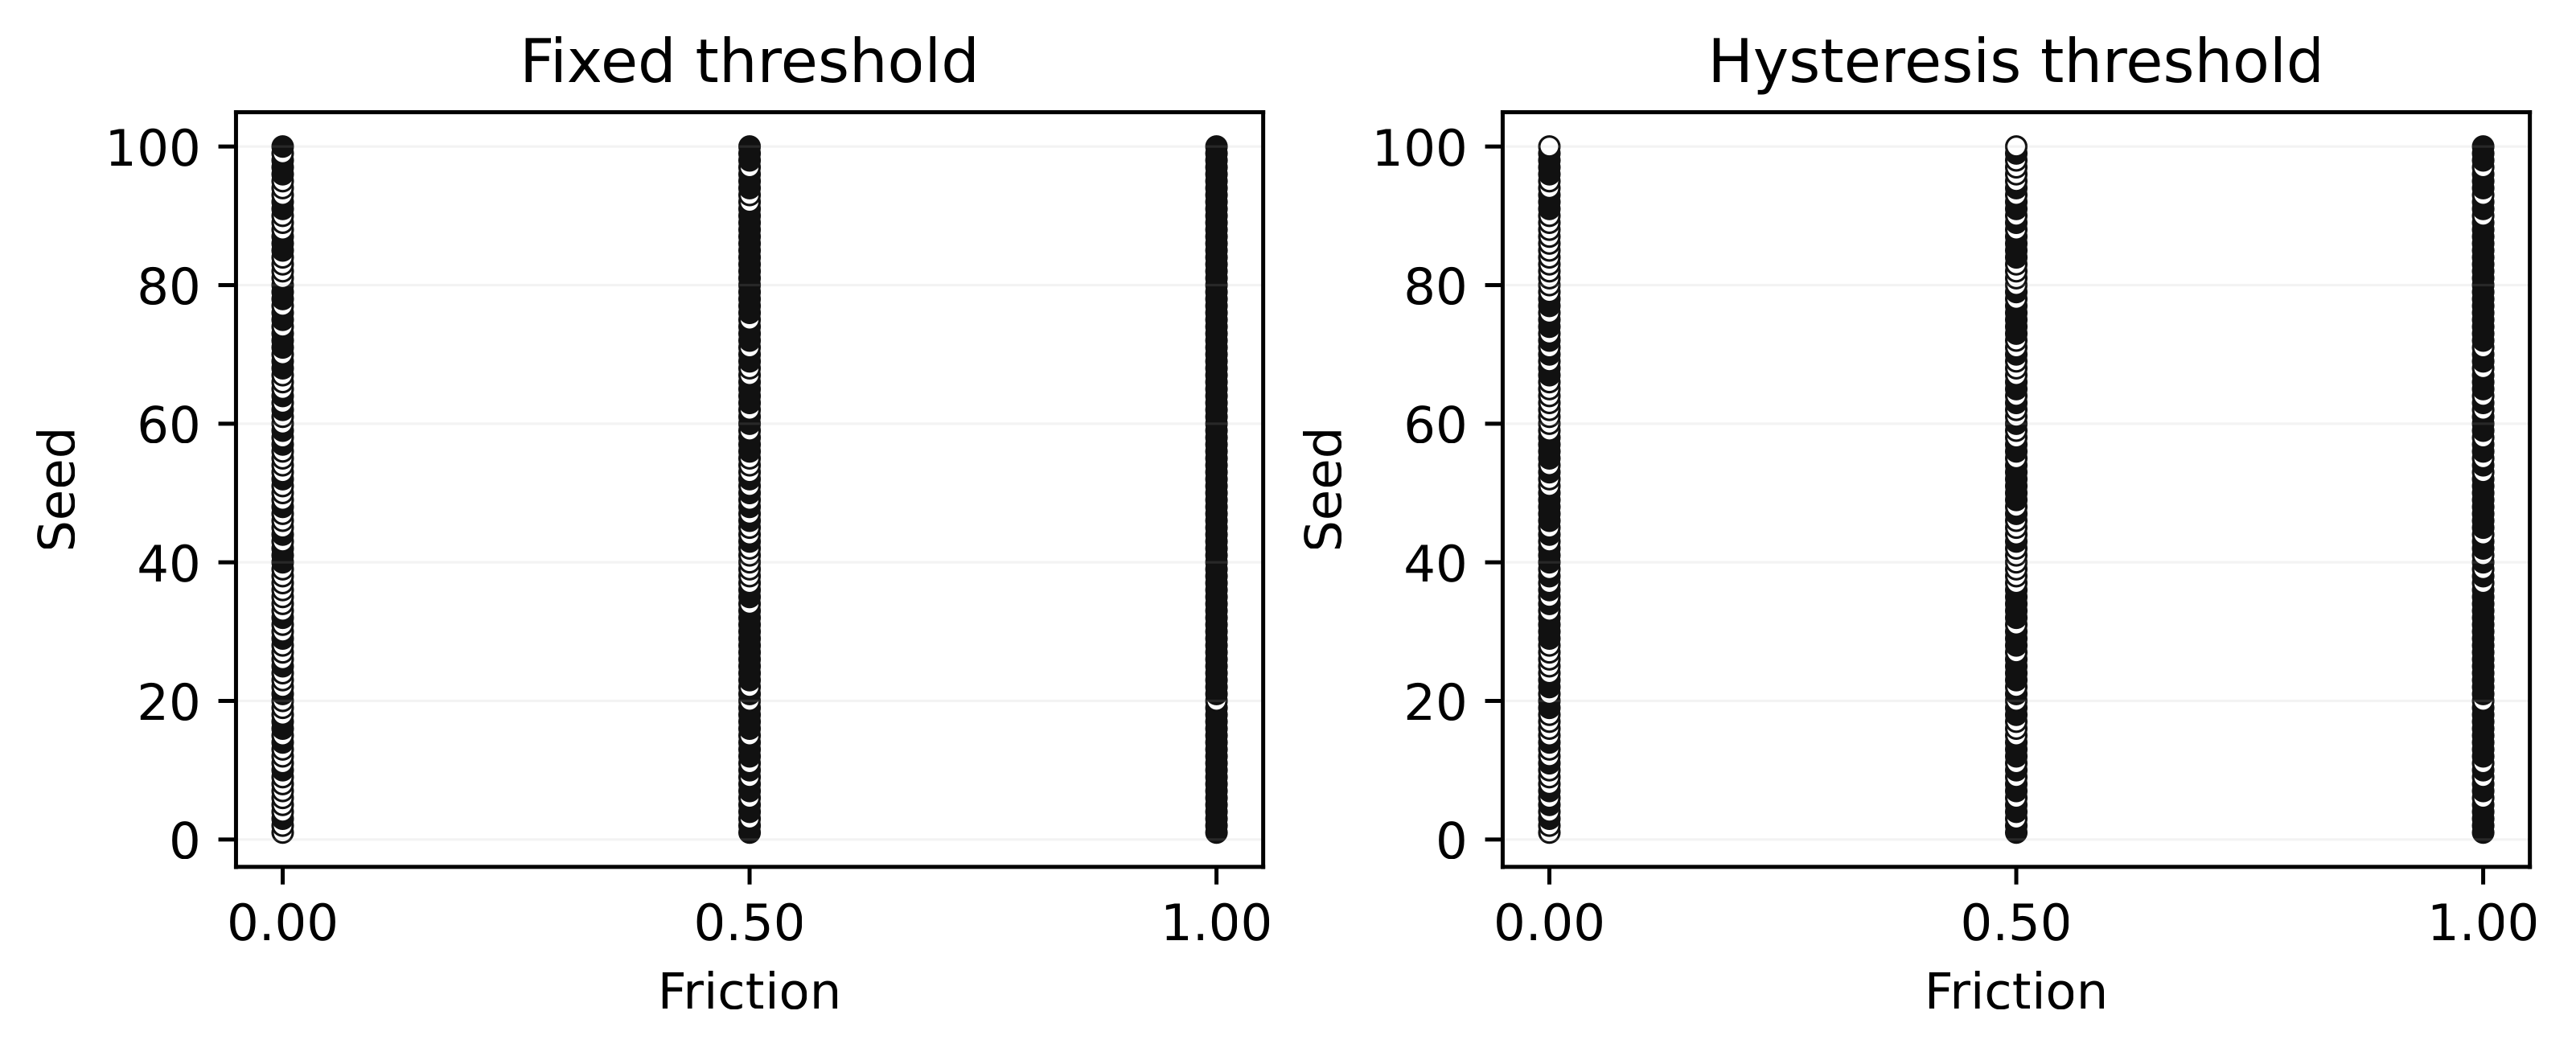
\includegraphics[width=\appwidefigwidth]{assets/figures/fig_event_micro_interface_seed_recurrence_appendix.png}
% \caption{Seed-level disagreement strips for event-micro interfaces. Each panel shows the same seed set under one fixed interface.}
% \label{fig:event-micro-interface-seed-recurrence}
% \end{figure}

\FloatBarrier

\section{Traffic Fixed-Budget Robustness}
\label{app:traffic-redesign}

\subsection{Interface/Friction Heatmap}

\begin{figure}[!htbp]
\centering
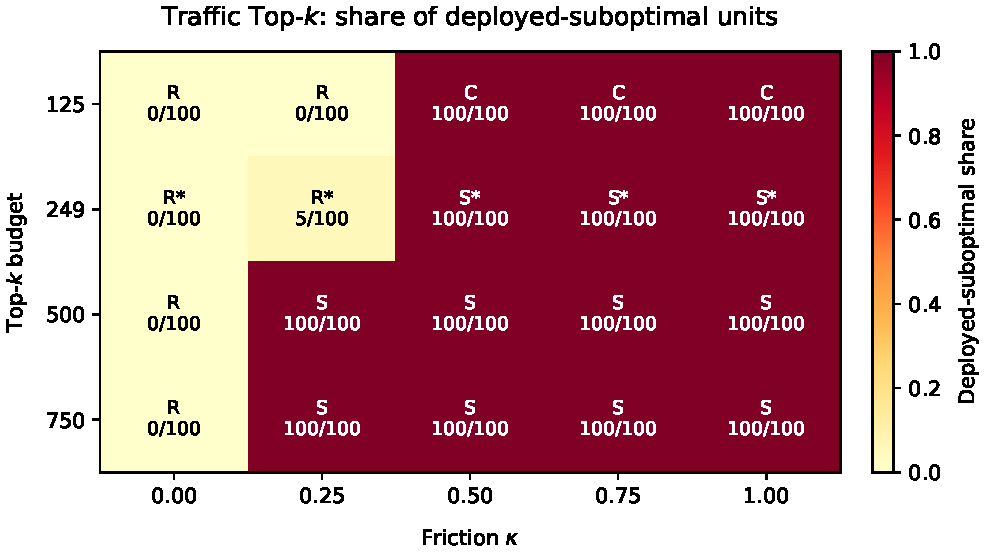
\includegraphics[width=0.84\linewidth]{results/fig_traffic_topk_heatmap.pdf}
\caption{Traffic Top-\(k\) across budgets and friction levels. Colors show the share of deployed-suboptimal units. Cell text reports the deployed winner label and deployed-suboptimal count; R = Reactive, S = Smoother, C = Calibrated, and * marks the canonical budget. All tested \(k\) values align at zero friction. At \(\kappa \ge 0.50\), every tested \(k \in \{125,249,500,750\}\) shows 100/100 deployed-suboptimality of the reactive offline-selected candidate. The \(\kappa=0.25\) column is mixed and is interpreted as a transition region.}
\label{fig:traffic-topk-heatmap}
\end{figure}

The heatmap replaces the older compact Top-\(k\) family table: it extends the grid to \(k=750\) and intermediate frictions \(\kappa\in\{0.25,0.75\}\), while showing that the canonical \(k=249\) point is not isolated.

\subsection{Temporal-Split Robustness}

\begin{table}[!htbp]
\centering
\scriptsize
\setlength{\tabcolsep}{2.5pt}
\begin{adjustbox}{width=\appwidetablewidth}
\begin{tabular}{llllllll}
\toprule
Split & \(\kappa\) & Offline sel. & Deploy winner & Subopt. & Mean shortfall & 95\% CI & Audit status \\
\midrule
Canonical & 0.00 & Reactive short & Reactive short & 0/100 & 0.000 & [0.000, 0.000] & Zero-friction aligned \\
Canonical & 0.50 & Reactive short & Lagged smoother & 100/100 & 10.177 & [9.871, 10.486] & Pass \\
Canonical & 1.00 & Reactive short & Lagged smoother & 100/100 & 31.300 & [30.823, 31.792] & Pass \\
Earlier & 0.00 & Reactive short & Reactive short & 0/100 & 0.000 & [0.000, 0.000] & Zero-friction aligned \\
Earlier & 0.50 & Reactive short & Lagged smoother & 100/100 & 9.152 & [8.821, 9.487] & Pass \\
Earlier & 1.00 & Reactive short & Lagged smoother & 100/100 & 27.861 & [27.312, 28.423] & Pass \\
Later & 0.00 & Reactive short & Reactive short & 0/100 & 0.000 & [0.000, 0.000] & Zero-friction aligned \\
Later & 0.50 & Reactive short & Lagged smoother & 100/100 & 11.963 & [11.654, 12.270] & Pass \\
Later & 1.00 & Reactive short & Lagged smoother & 100/100 & 35.243 & [34.764, 35.721] & Pass \\
\bottomrule
\end{tabular}

\end{adjustbox}
\caption{Traffic-Hourly temporal-split robustness. Each split recomputes the offline-selected model from that split's validation segment. Zero-friction rows are marked as alignment checks; positive-friction rows are marked Pass when the split preserves zero-friction alignment and shows recurrent deployed-suboptimality with positive paired shortfalls.}
\label{tab:traffic-temporal-splits}
\end{table}

Event-micro temporal slices show positive-friction recurrence but fail the clean zero-friction split-alignment gate, so they are retained only as secondary audit context. Predefined Traffic time-of-day and relative-rank checks were also run as secondary slices, but the temporal-split and interface/friction diagnostics provide cleaner fixed-budget robustness evidence.

\FloatBarrier

\section{Replay-Based Deployed-Feedback Reselection}
\label{app:reselection-diagnostic}

This diagnostic asks whether a small calibration segment of deployed-feedback replay can reduce or correct an offline model-selection error within the same fixed candidate set and interface. It is not an online learning or exploration algorithm: it assumes replay access to held-out outcomes for all fixed-interface candidates and is used only as an appendix diagnostic. Calibration is always the earlier segment and evaluation is always the later segment; no future deployed utility from the evaluation segment is used when selecting the reselected candidate.

For compactness, Table~\ref{tab:reselection-diagnostic} reports representative budget rows, including the lower-friction Event boundary case and the high-friction/Traffic cases that pass the diagnostic; the full budget grid remains in the isolated experiment report.

\begin{table}[!htbp]
\centering
\begin{minipage}{\appmidtablewidth}
\centering
\scriptsize
\setlength{\tabcolsep}{2.5pt}
\begin{adjustbox}{width=\linewidth}
\begin{tabular}{lccccccc}
\toprule
Domain & \(\kappa\) & Budget & Reduction & Resel. subopt. & Correction & Worse & Diagnostic status \\
\midrule
Event & 0.50 & 20\% & 28.7\% & 59\% & 41\% & 26\% & Boundary \\
Event & 1.00 & 10\% & 78.8\% & 30\% & 70\% & 2\% & Pass \\
Traffic & 0.50 & 10\% & 100\% & 0\% & 100\% & 0\% & Pass \\
Traffic & 1.00 & 10\% & 100\% & 0\% & 100\% & 0\% & Pass \\
\bottomrule
\end{tabular}

\end{adjustbox}
\caption{Replay-based deployed-feedback reselection diagnostic. This diagnostic assumes replay access to held-out outcomes for all fixed-interface candidates and is not a deploy-one-policy online learning algorithm. The lower-friction Event row is retained as a Boundary case: it improves shortfall but has nontrivial worse-than-offline share, so it is not used as primary support.}
\label{tab:reselection-diagnostic}
\end{minipage}
\end{table}

\FloatBarrier

\section{Candidate-Pool and Residual-Audit Checks}
\label{app:candidate-residual-checks}

\subsection{Stronger Candidate-Pool Fairness Pilot}
\label{app:stronger-pool-pilot}

This pilot checks whether the selection-transfer mismatch disappears under lightweight added candidates. It is not a forecasting model benchmark and uses fixed, lightweight configurations without extensive hyperparameter search.

\begin{table}[!htbp]
\centering
\begin{minipage}{\appmidtablewidth}
\centering
\scriptsize
\setlength{\tabcolsep}{2.5pt}
\begin{adjustbox}{width=\linewidth}
\begin{tabular}{lllllll}
\toprule
Domain & \(\kappa\) & Added candidates & Offline sel. & Deploy winner & Subopt. & Mean shortfall \\
\midrule
Event & 0.50 & Logit/cal. logit/GBDT & Reactive sharp & Calibrated baseline & 82/100 & 0.01884 \\
Event & 1.00 & Logit/cal. logit/GBDT & Reactive sharp & Lagged smoother & 97/100 & 0.06035 \\
Traffic & 0.50 & Linear AR head & Reactive short & Lagged smoother & 100/100 & 10.17694 \\
Traffic & 1.00 & Linear AR head & Reactive short & Lagged smoother & 100/100 & 31.29953 \\
\bottomrule
\end{tabular}

\end{adjustbox}
\caption{Expanded candidate-pool pilot. The qualitative selection-transfer mismatch remains under lightweight added candidates, but this check is appendix-only because the paper does not aim to benchmark forecasting model classes.}
\label{tab:stronger-pool-pilot}
\end{minipage}
\end{table}

\subsection{Residual-Warning Audit Family}
\label{app:residual-audit}

We use this family as audit context rather than main-domain breadth: EPA, Capital Bikeshare, and Wikimedia satisfy the residual-audit alignment and recurrence checks, while NYC TLC and M5 fail the zero-friction alignment gate.

\begin{table}[!htbp]
\centering
\begin{minipage}{\appmidtablewidth}
\centering
\scriptsize
\setlength{\tabcolsep}{2.5pt}
\begin{adjustbox}{width=\linewidth}
\begin{tabular}{lcrrrrl}
\toprule
Candidate & Audit status & Units & Zero subopt. & Positive subopt. & Mean shortfall & Placement \\
\midrule
EPA AQS PM2.5 & Pass & 16 & 0.000 & 1.000 & 486.94 & Appendix summary \\
Capital Bikeshare & Pass & 16 & 0.063 & 1.000 & 2791.75 & Appendix summary \\
Wikimedia hourly & Pass & 11 & 0.000 & 1.000 & 118.18 & Appendix summary \\
NYC TLC taxi-zone & Fail & 16 & 0.750 & 1.000 & 2285.81 & Failed-gate context \\
M5 store-quota & Fail & 20 & 0.500 & 0.900 & 24.15 & Failed-gate context \\
\bottomrule
\end{tabular}

\end{adjustbox}
\caption{Residual-warning audit family. EPA, Capital Bikeshare, and Wikimedia satisfy the residual-audit alignment and recurrence checks and remain appendix summary context; NYC TLC and M5 fail the zero-friction alignment gate and are retained as failed-gate context. These rows are not promoted as main-domain breadth.}
\label{tab:residual-candidate-audit}
\end{minipage}
\end{table}

\FloatBarrier

\section{Mechanism, Tie Audit, and Secondary Corroboration}
\label{app:mechanism-tie-secondary}

Inventory remains operational corroboration rather than a main-domain breadth claim: the main text reports the high-friction replenishment row, while mixed zero/low-friction and expanded-family inventory checks are retained only as secondary context. Load-following is likewise reduced to failed-gate context because its lower-margin rows are tie-sensitive or partially sensitive. Predefined Traffic time-of-day and relative-rank variants are not used as paper-facing robustness now that the temporal-split and interface/friction diagnostics provide cleaner fixed-budget evidence.

\subsection{Mechanism Check under Fixed Action Paths}

Q1 serves only as mechanism support for why selection-transfer divergence can arise. Holding the proposed action path fixed, synthetic and inventory show how a fixed interface can separate proposed and realized actions once friction is introduced.

\begin{figure}[!htbp]
\centering
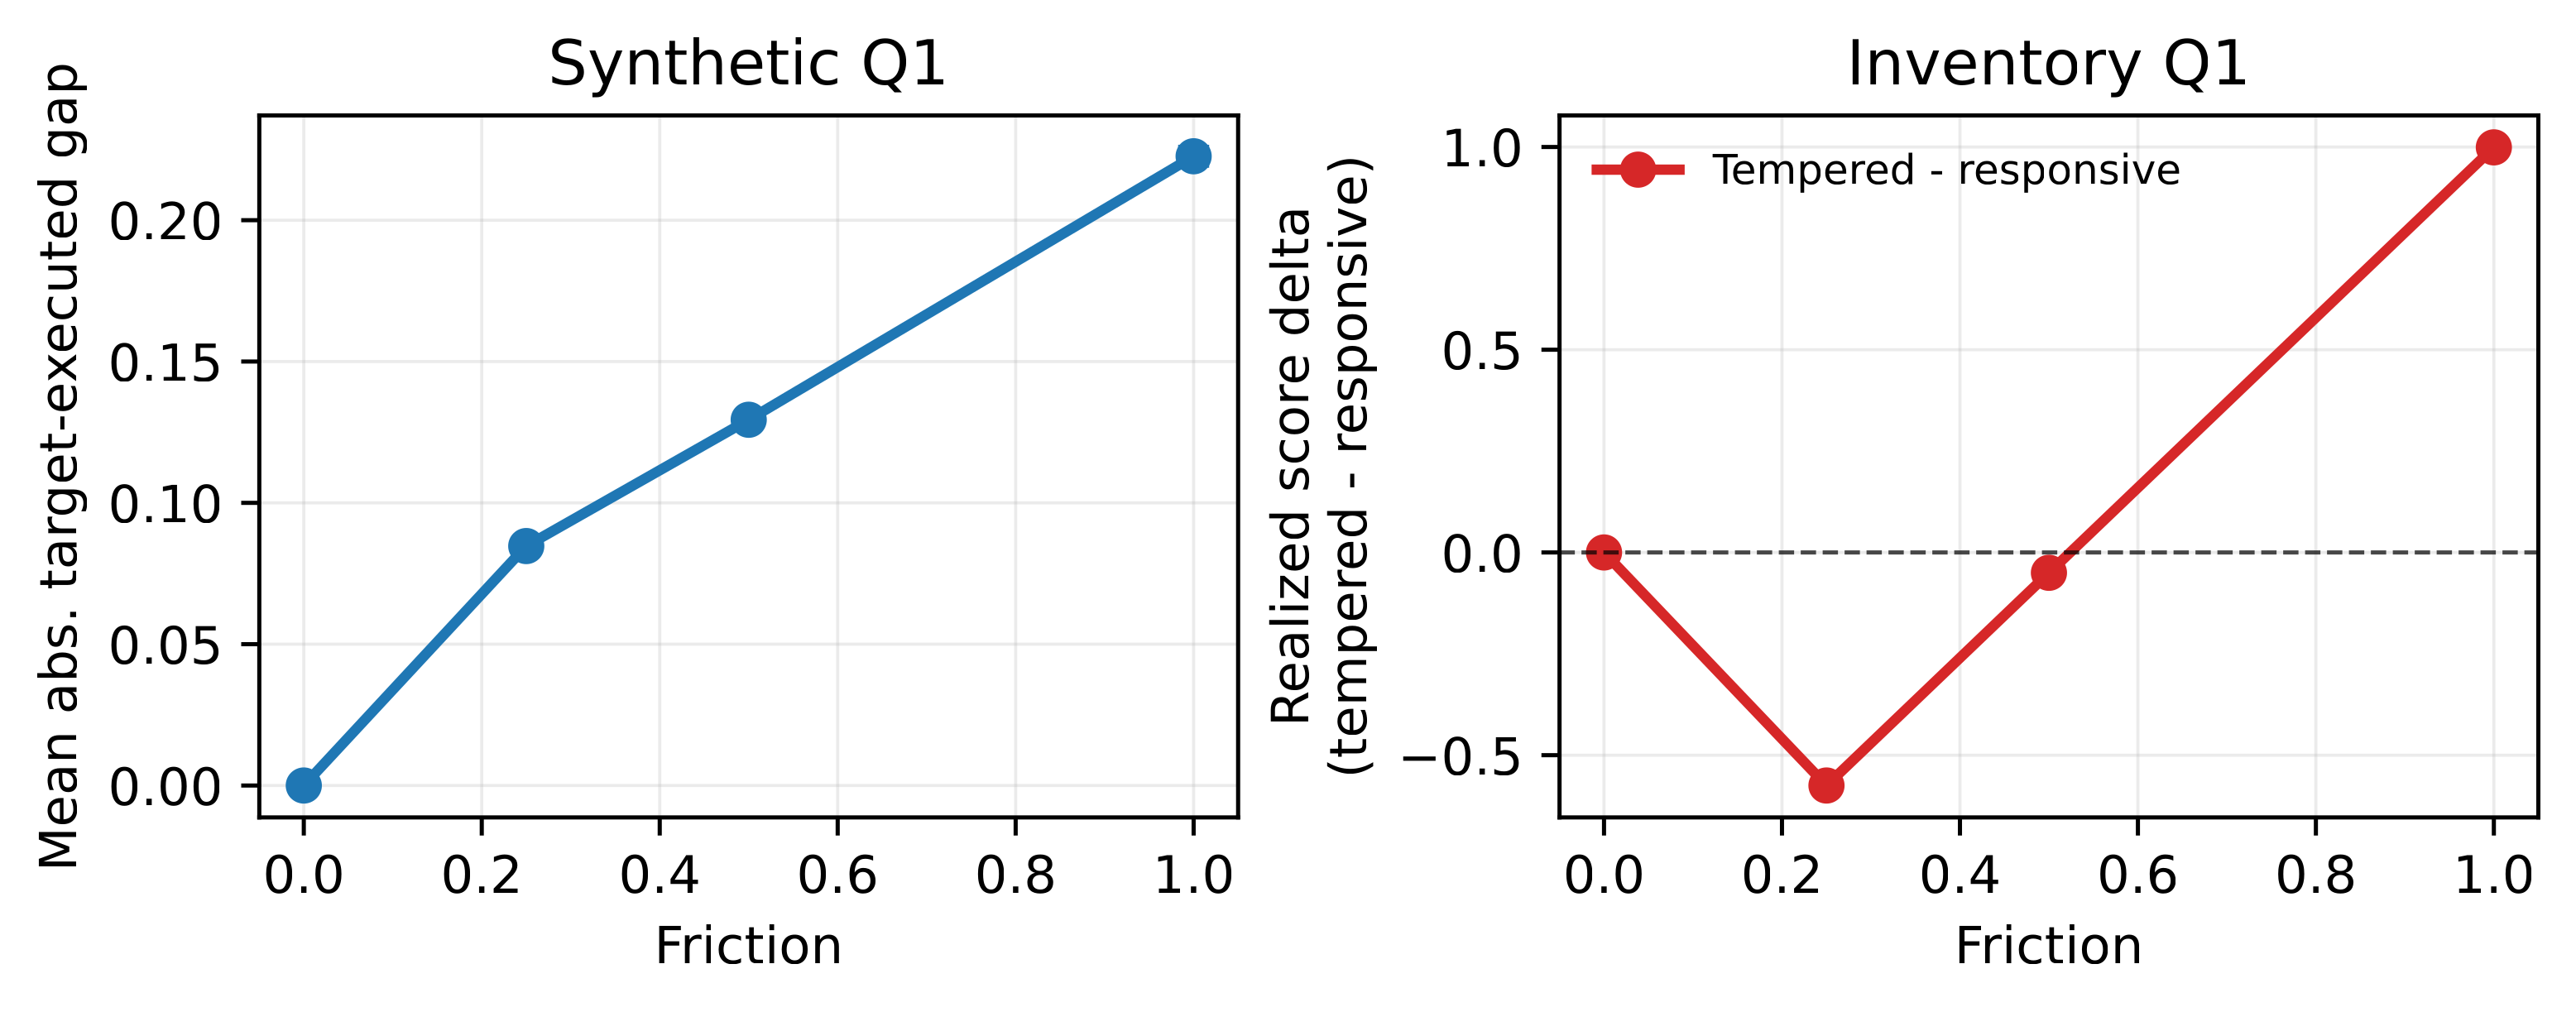
\includegraphics[width=0.64\linewidth]{assets/figures/fig_q1_results_v2.png}
\caption{Q1 mechanism support. Even with the same proposed actions, a fixed frictional interface can alter realized actions and realized score. This illustrates how a fixed deployment interface can change the realized utility ordering of offline-selected candidates.}
\label{fig:q1-required}
\end{figure}

\FloatBarrier

\subsection{Uncertainty and \(\epsilon\)-Tie Audit}
\label{app:uncertainty-reporting}

This appendix reports uncertainty for the seed-level recurrence and paired deployed-shortfall summaries used in the main report card. We emphasize intervals and paired shortfalls rather than hypothesis-test significance. For continuous deployed shortfalls, we use 10,000 paired seed bootstrap resamples. For binary share summaries, rows with fewer than 30 matched seeds use Clopper--Pearson exact intervals; rows with at least 30 matched seeds use Wilson intervals. We report these intervals as descriptive uncertainty summaries for the reporting diagnostic, not as hypothesis-test evidence for a broader population-level claim.

\begin{table}[!htbp]
\centering
\scriptsize
\setlength{\tabcolsep}{2.5pt}
\begin{adjustbox}{width=\appwidetablewidth}
\begin{tabular}{llllllll}
\toprule
Domain & Interface & $\kappa$ & Seeds & Agree. & Subopt. share/count & Subopt. 95\% CI & CI type \\
\midrule
Event-micro & threshold $\tau=0.55$ & 0.50 & 100 & 0.31 & 0.69 (69/100) & [0.594, 0.772] & Wilson \\
Event-micro & threshold $\tau=0.55$ & 1.00 & 100 & 0.01 & 0.99 (99/100) & [0.946, 0.998] & Wilson \\
Traffic Top-\(k\) & budget $k=249$ & 0.50 & 100 & 0.00 & 1.00 (100/100) & [0.963, 1.000] & Wilson \\
Traffic Top-\(k\) & budget $k=249$ & 1.00 & 100 & 0.00 & 1.00 (100/100) & [0.963, 1.000] & Wilson \\
Inventory & replenishment & 0.50 & 100 & 0.26 & 0.74 (74/100) & [0.646, 0.816] & Wilson \\
Inventory & replenishment & 1.00 & 100 & 0.01 & 0.99 (99/100) & [0.946, 0.998] & Wilson \\
\bottomrule
\end{tabular}

\end{adjustbox}
\caption{Seed-level recurrence and share uncertainty for deployed-suboptimality. Agreement rate is the fraction of matched seeds for which the offline-selected model is also the deployed-utility best model; deployed-suboptimal share is the complementary fraction. We report Clopper--Pearson exact intervals for rows with $n<30$ and Wilson intervals otherwise.}
\label{tab:q2-recurrence-share-ci}
\end{table}

Aggregate recurrence intervals and uncertainty bands summarize the seed-level pattern without the dense seed-strip visualization.

\begin{table}[!htbp]
\centering
\scriptsize
\setlength{\tabcolsep}{2.5pt}
\begin{adjustbox}{width=\appwidetablewidth}
\begin{tabular}{llllll}
\toprule
Domain & Friction & Mean deployed gap & Mean gap 95\% bootstrap CI & Median deployed gap & Median gap 95\% bootstrap CI \\
\midrule
Event micro & 0.50 & 0.011 & [0.009, 0.014] & 0.008 & [0.004, 0.011] \\
Event micro & 1.00 & 0.057 & [0.052, 0.063] & 0.053 & [0.048, 0.059] \\
Traffic-Hourly Top-k & 0.50 & 7.016 & [6.756, 7.283] & 6.977 & [6.706, 7.281] \\
Traffic-Hourly Top-k & 1.00 & 24.651 & [24.226, 25.079] & 24.473 & [24.001, 25.051] \\
Inventory & 0.50 & 0.240 & [0.195, 0.286] & 0.202 & [0.154, 0.256] \\
Inventory & 1.00 & 1.029 & [0.946, 1.111] & 1.045 & [0.926, 1.167] \\
Load-following & 0.25 & 0.001 & [0.000, 0.001] & 0.000 & [0.000, 0.001] \\
Load-following & 0.50 & 0.001 & [0.000, 0.002] & 0.001 & [0.000, 0.002] \\
Load-following & 1.00 & 0.002 & [0.001, 0.005] & 0.002 & [0.000, 0.003] \\
\bottomrule
\end{tabular}

\end{adjustbox}
\caption{Paired-bootstrap intervals for deployed-shortfall rows. Deployed shortfall is the paired deployed-utility shortfall $U_{\mathrm{best}} - U_{\mathrm{offline\mbox{-}selected}}$ computed within each matched seed. Intervals use 10,000 paired seed bootstrap resamples. Event-micro and Traffic-Hourly provide the main prediction-to-decision selection-transfer evidence; inventory is operational corroboration.}
\label{tab:q2-gap-bootstrap-cis}
\end{table}

\begin{figure}[!htbp]
\centering
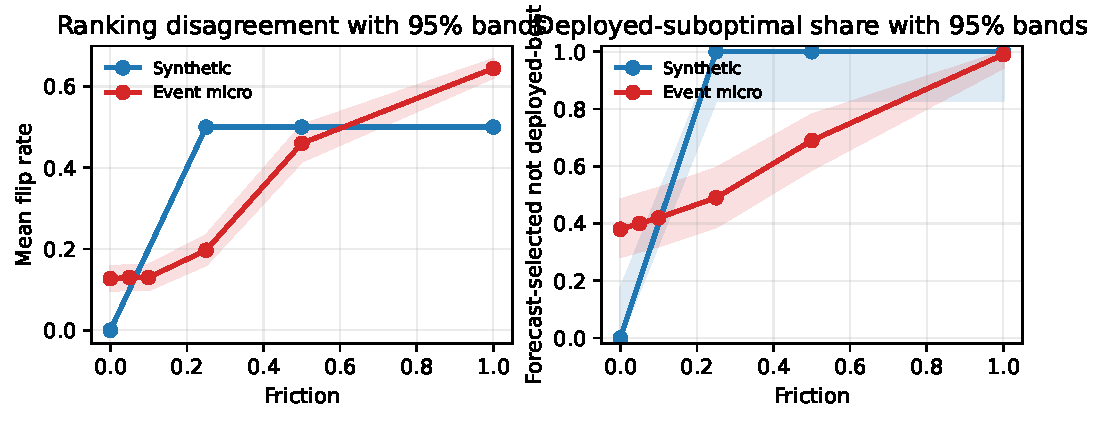
\includegraphics[width=0.84\linewidth]{assets/figures/fig_q2_uncertainty_appendix.pdf}
\caption{Selection-transfer uncertainty summaries for synthetic and event-micro. Left: flip rate; right: deployed-suboptimal share. Bands follow the interval convention described in Appendix~\ref{app:uncertainty-reporting}; zero-width bands may coincide with the line.}
\label{fig:q2-uncertainty}
\end{figure}

\FloatBarrier

\subsection{Epsilon-Tie Sensitivity}

The audit covers the gated report-card domains and is used to check whether deployed-suboptimality survives small relative tie thresholds.

\begin{table}[H]
\caption{\(\epsilon\)-tie sensitivity for the gated report-card domains. A seed is tie-compatible when the deployed shortfall of the offline-selected model is at most \(\epsilon_{\mathrm{rel}}S + 10^{-12}\), where \(S\) is the median seed-level deployed-utility scale within the row. The Tie status column records whether the deployed-suboptimality conclusion remains after applying the stated relative tie threshold; it is a descriptive robustness label, not a hypothesis-test outcome.}
\label{tab:epsilon-tie-sensitivity}
\centering
\scriptsize
\setlength{\tabcolsep}{2.2pt}
\begin{adjustbox}{width=\appwidetablewidth}
\input{results/table_epsilon_tie_sensitivity_gated.tex}
\end{adjustbox}
\end{table}

% Removed from compiled appendix: dense seed-strip.
% Aggregate recurrence and uncertainty evidence are reported in Table~\ref{tab:q2-recurrence-share-ci} and Figure~\ref{fig:q2-uncertainty}.
% \begin{figure}[!htbp]
% \centering
% 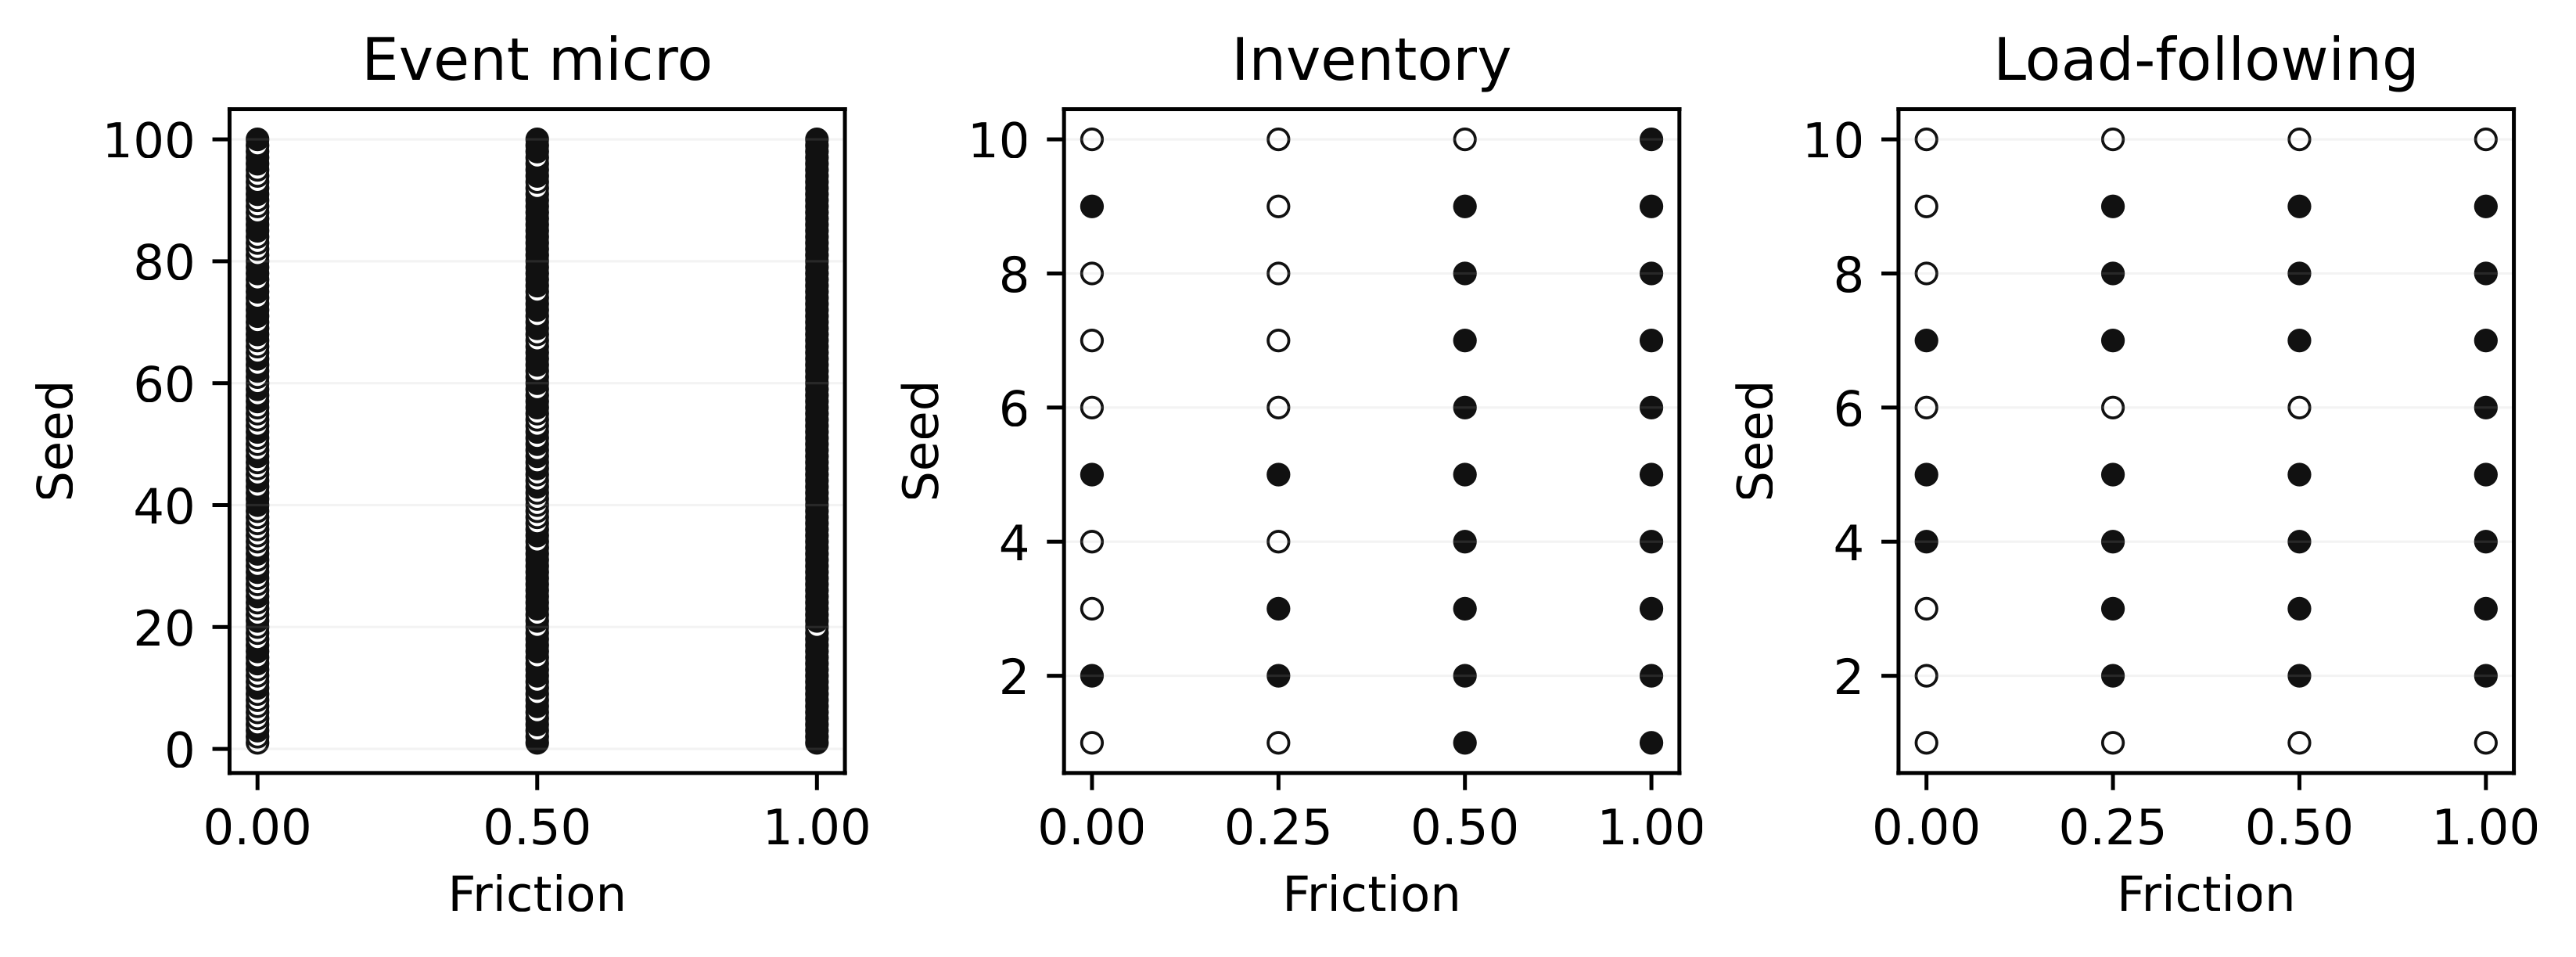
\includegraphics[width=\appwidefigwidth]{assets/figures/fig_q2_seed_recurrence_appendix.png}
% \caption{Seed-level disagreement strips for the main Q2 domains. Filled markers indicate seeds where the offline-selected model is not deployed-best under the fixed interface.}
% \label{fig:q2-seed-recurrence}
% \end{figure}

\FloatBarrier

\end{document}
